\section{Hardware/software mapping}

Our Calendar system is run by two devices. The user program run on the user computer, and the synchronized parts will be on the server together with our share system. The two devices will have a connection to each other, we have not yet decided which kind of connection it would be.

\begin{figure}[h]
\centering
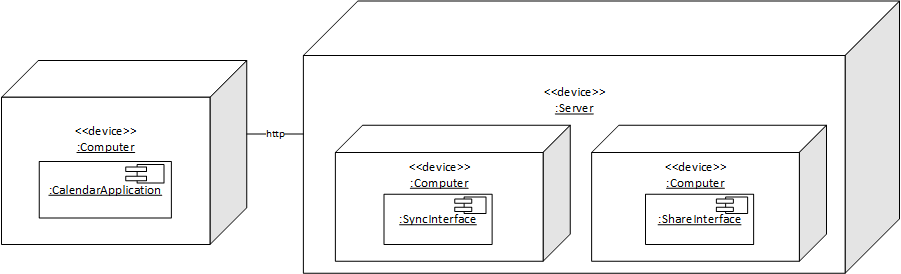
\includegraphics[width=160mm]{UMLDeployment.png}
\caption{UML Deployment diagram \label{overflow}}
\label{figur:UMLDeployment}
\end{figure}

Now that we have mapped our program to the hardware that is used to run our system we dicovered that some informations had to be handled between the computer and the server. Therefore we have made up a Component Diagram with the subsystems. If we study the ‘CalendarManagement’ the ‘SyncSubsystem’ and the ‘ShareSubsystem’, we find that classes related to synchronization and share have been kept seperated. The information from Model in CalendarManagement have to be transfered from the computer to the server via a network connection. The Controller in ‘CalendarManagement’ handles the communication between ‘CalendarManagement’ and ‘SyncSubsystem’ \& ‘ShareSubsystem’.